% questions.tex —— 2003 年·江苏卷 · 题目内容片段（无答案）
% 由 tools/generate_projects.py 依来源总账自 2003/2003_数学真题_江苏_试题.md 生成，勿手改（改源 MD 后重跑）


\begin{gktip}
\textbf{来源说明}：本题面依据固定源 PDF《2003 普通高等学校招生考试 (江苏卷)》逐题核对转录。固定源为 2 页 A3 横向扫描排印，原卷印刷页码 131–132；PDF 不含答案或解析页。
\end{gktip}

\Needspace{0.4\textheight}
\begin{question}
\gkti{1}如果函数 $y = ax^2 + bx + a$ 的图象与 $x$ 轴有两个交点，则点 $(a, b)$ 在 $aOb$ 平面上的区域（不包含边界）为\mbox{（　　）}
\nopagebreak[4]
\begin{center}% 2003 年江苏卷第 1 题：点 (a, b) 区域选项图
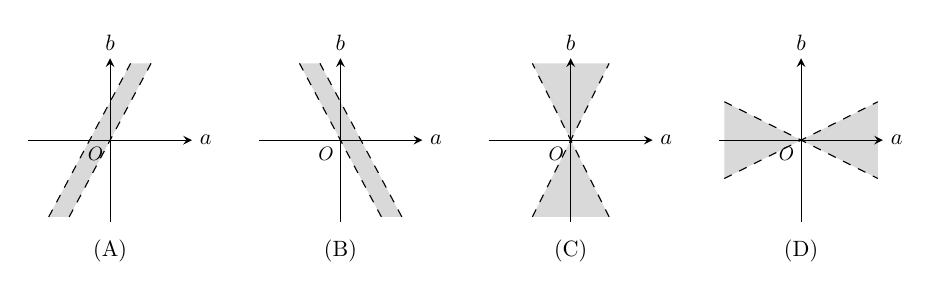
\begin{tikzpicture}[>=stealth,scale=0.65]
  % A
  \begin{scope}[shift={(0,0)}]
    \fill[black!15] (-1.2,-1.5) -- (-0.8,-1.5) -- (0.8,1.5) -- (0.4,1.5) -- cycle;
    \draw[->] (-1.6,0) -- (1.6,0) node[right,scale=0.8] {$a$};
    \draw[->] (0,-1.6) -- (0,1.6) node[above,scale=0.8] {$b$};
    \node[below left,scale=0.7] at (0,0) {$O$};
    \draw[dashed] (-1.2,-1.5) -- (0.4,1.5);
    \draw[dashed] (-0.8,-1.5) -- (0.8,1.5);
    \node[below,scale=0.8] at (0,-1.8) {(A)};
  \end{scope}

  % B
  \begin{scope}[shift={(4.5,0)}]
    \fill[black!15] (1.2,-1.5) -- (0.8,-1.5) -- (-0.8,1.5) -- (-0.4,1.5) -- cycle;
    \draw[->] (-1.6,0) -- (1.6,0) node[right,scale=0.8] {$a$};
    \draw[->] (0,-1.6) -- (0,1.6) node[above,scale=0.8] {$b$};
    \node[below left,scale=0.7] at (0,0) {$O$};
    \draw[dashed] (1.2,-1.5) -- (-0.4,1.5);
    \draw[dashed] (0.8,-1.5) -- (-0.8,1.5);
    \node[below,scale=0.8] at (0,-1.8) {(B)};
  \end{scope}

  % C
  \begin{scope}[shift={(9,0)}]
    \fill[black!15] (0,0) -- (0.75,1.5) -- (-0.75,1.5) -- cycle;
    \fill[black!15] (0,0) -- (0.75,-1.5) -- (-0.75,-1.5) -- cycle;
    \draw[->] (-1.6,0) -- (1.6,0) node[right,scale=0.8] {$a$};
    \draw[->] (0,-1.6) -- (0,1.6) node[above,scale=0.8] {$b$};
    \node[below left,scale=0.7] at (0,0) {$O$};
    \draw[dashed] (-0.75,-1.5) -- (0.75,1.5);
    \draw[dashed] (0.75,-1.5) -- (-0.75,1.5);
    \node[below,scale=0.8] at (0,-1.8) {(C)};
  \end{scope}

  % D
  \begin{scope}[shift={(13.5,0)}]
    \fill[black!15] (0,0) -- (1.5,0.75) -- (1.5,-0.75) -- cycle;
    \fill[black!15] (0,0) -- (-1.5,0.75) -- (-1.5,-0.75) -- cycle;
    \draw[->] (-1.6,0) -- (1.6,0) node[right,scale=0.8] {$a$};
    \draw[->] (0,-1.6) -- (0,1.6) node[above,scale=0.8] {$b$};
    \node[below left,scale=0.7] at (0,0) {$O$};
    \draw[dashed] (-1.5,-0.75) -- (1.5,0.75);
    \draw[dashed] (-1.5,0.75) -- (1.5,-0.75);
    \node[below,scale=0.8] at (0,-1.8) {(D)};
  \end{scope}
\end{tikzpicture}
\end{center}
\nopagebreak[4]
（A）A　　（B）B　　（C）C　　（D）D

\end{question}
\begin{question}
\gkti{2}抛物线 $y = ax^2$ 的准线方程是 $y = 2$，则 $a$ 的值为\mbox{（　　）}

（A）$\dfrac{1}{8}$　　（B）$-\dfrac{1}{8}$　　（C）8　　（D）$-8$

\end{question}
\begin{question}
\gkti{3}已知 $x \in \left(-\dfrac{\pi}{2}, 0\right)$，$\cos x = \dfrac{4}{5}$，则 $\tan 2x =$\mbox{（　　）}

（A）$\dfrac{7}{24}$　　（B）$-\dfrac{7}{24}$　　（C）$\dfrac{24}{7}$　　（D）$-\dfrac{24}{7}$

\end{question}
\begin{question}
\gkti{4}设函数
\nopagebreak[4]
\[f(x) = \begin{cases} 2^{-x} - 1, & x \le 0, \\ x^{\frac{1}{2}}, & x > 0, \end{cases}\]
若 $f(x_0) > 1$，则 $x_0$ 的取值范围是\mbox{（　　）}

（A）$(-1, 1)$　　（B）$(-1, +\infty)$　　（C）$(-\infty, -2) \cup (0, +\infty)$　　（D）$(-\infty, -1) \cup (1, +\infty)$

\end{question}
\begin{question}
\gkti{5}$O$ 是平面上一定点，$A$、$B$、$C$ 是平面上不共线的三个点，动点 $P$ 满足
\nopagebreak[4]
\[\vec{OP} = \vec{OA} + \lambda \left(\frac{\vec{AB}}{|\vec{AB}|} + \frac{\vec{AC}}{|\vec{AC}|}\right), \quad \lambda \in [0, +\infty),\]
则 $P$ 的轨迹一定通过 $\triangle ABC$ 的\mbox{（　　）}

（A）外心　　（B）内心　　（C）重心　　（D）垂心

\end{question}
\begin{question}
\gkti{6}函数 $y = \ln\dfrac{x+1}{x-1}$，$x \in (1, +\infty)$ 的反函数为\mbox{（　　）}

（A）$y = \dfrac{\mathrm{e}^x - 1}{\mathrm{e}^x + 1}$，$x \in (0, +\infty)$　　（B）$y = \dfrac{\mathrm{e}^x + 1}{\mathrm{e}^x - 1}$，$x \in (0, +\infty)$

（C）$y = \dfrac{\mathrm{e}^x - 1}{\mathrm{e}^x + 1}$，$x \in (-\infty, 0)$　　（D）$y = \dfrac{\mathrm{e}^x + 1}{\mathrm{e}^x - 1}$，$x \in (-\infty, 0)$

\end{question}
\begin{question}
\gkti{7}棱长为 $a$ 的正方体中，连结相邻面的中心，以这些线段为棱的八面体的体积为\mbox{（　　）}

（A）$\dfrac{a^3}{3}$　　（B）$\dfrac{a^3}{4}$　　（C）$\dfrac{a^3}{6}$　　（D）$\dfrac{a^3}{12}$

\end{question}
\begin{question}
\gkti{8}设 $a > 0$，$f(x) = ax^2 + bx + c$，曲线 $y = f(x)$ 在点 $P(x_0, f(x_0))$ 处切线的倾斜角的取值范围为 $\left[0, \dfrac{\pi}{4}\right]$，则 $P$ 到曲线 $y = f(x)$ 对称轴距离的取值范围为\mbox{（　　）}

（A）$\left[0, \dfrac{1}{a}\right]$　　（B）$\left[0, \dfrac{1}{2a}\right]$　　（C）$\left[0, \left|\dfrac{b}{2a}\right|\right]$　　（D）$\left[0, \left|\dfrac{b-1}{2a}\right|\right]$

\end{question}
\begin{question}
\gkti{9}已知方程 $(x^2 - 2x + m)(x^2 - 2x + n) = 0$ 的四个根组成一个首项为 $\dfrac{1}{4}$ 的等差数列，则 $|m - n| = $\mbox{（　　）}

（A）1　　（B）$\dfrac{3}{4}$　　（C）$\dfrac{1}{2}$　　（D）$\dfrac{3}{8}$

\end{question}
\begin{question}
\gkti{10}已知双曲线中心在原点且一个焦点为 $F(\sqrt{7}, 0)$，直线 $y = x - 1$ 与其相交于 $M$、$N$ 两点，$MN$ 中点的横坐标为 $-\dfrac{2}{3}$，则此双曲线的方程是\mbox{（　　）}

（A）$\dfrac{x^2}{3} - \dfrac{y^2}{4} = 1$　　（B）$\dfrac{x^2}{4} - \dfrac{y^2}{3} = 1$　　（C）$\dfrac{x^2}{5} - \dfrac{y^2}{2} = 1$　　（D）$\dfrac{x^2}{2} - \dfrac{y^2}{5} = 1$

\end{question}
\begin{question}
\gkti{11}已知长方形的四个顶点 $A(0, 0)$，$B(2, 0)$，$C(2, 1)$ 和 $D(0, 1)$，一质点从 $AB$ 的中点 $P_0$ 沿与 $AB$ 的夹角 $\theta$ 的方向射到 $BC$ 上的点 $P_1$ 后，依次反射到 $CD$、$DA$ 和 $AB$ 上的点 $P_2$、$P_3$ 和 $P_4$（入射角等于反射角），设 $P_4$ 的坐标为 $(x_4, 0)$，若 $1 < x_4 < 2$，则 $\tan\theta$ 的取值范围是\mbox{（　　）}

（A）$\left(\dfrac{1}{3}, 1\right)$　　（B）$\left(\dfrac{1}{3}, \dfrac{2}{3}\right)$　　（C）$\left(\dfrac{2}{5}, \dfrac{1}{2}\right)$　　（D）$\left(\dfrac{2}{5}, \dfrac{2}{3}\right)$

\end{question}
\begin{question}
\gkti{12}一个四面体的所有棱长都为 $\sqrt{2}$，四个顶点在同一球面上，则此球的表面积为\mbox{（　　）}

（A）$3\pi$　　（B）$4\pi$　　（C）$3\sqrt{3}\pi$　　（D）$6\pi$

\end{question}
\begin{question}
\gkti{13}$\left(x^2 - \dfrac{1}{2x}\right)^9$ 的展开式中 $x^9$ 系数是 $\underline{\hspace{2em}}$．

\end{question}
\begin{question}
\gkti{14}某公司生产三种型号的轿车，产量分别为 1200 辆，6000 辆和 2000 辆．为检验该公司的产品质量，现用分层抽样的方法抽取 46 辆进行检验，这三种型号的轿车依次应抽取 $\underline{\hspace{2em}}$，$\underline{\hspace{2em}}$，$\underline{\hspace{2em}}$ 辆．

\Needspace{0.4\textheight}
\end{question}
\begin{question}
\gkti{15}某城市在中心广场建造一个花圃，花圃分为 6 个部分（如图）．现要栽种 4 种不同颜色的花，每部分栽种一种且相邻部分不能栽种同样颜色的花，不同的栽种方法有 $\underline{\hspace{2em}}$ 种．（以数字作答）
\nopagebreak[4]
\begin{center}% 2003 年江苏卷第 15 题：花圃 6 个部分示意图
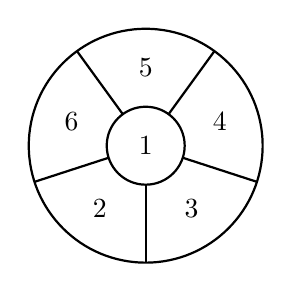
\begin{tikzpicture}[>=stealth,scale=0.9]
  \def\rIn{0.55}
  \def\rOut{1.65}
  % Circles
  \draw[thick] (0,0) circle (\rIn);
  \draw[thick] (0,0) circle (\rOut);
  
  % Radial lines
  \foreach \ang in {54, 126, 198, 270, 342} {
    \draw[thick] (\ang:\rIn) -- (\ang:\rOut);
  }
  
  % Labels
  \node at (0,0) {$1$};
  \node at (234:1.1) {$2$};
  \node at (306:1.1) {$3$};
  \node at (18:1.1) {$4$};
  \node at (90:1.1) {$5$};
  \node at (162:1.1) {$6$};
\end{tikzpicture}
\end{center}
\nopagebreak[4]
\end{question}
\begin{question}
\gkti{16}对于四面体 $ABCD$，给出下列四个命题：
① 若 $AB = AC$，$BD = CD$，则 $BC \perp AD$；
② 若 $AB = CD$，$AC = BD$，则 $BC \perp AD$；
③ 若 $AB \perp AC$，$BD \perp CD$，则 $BC \perp AD$；
④ 若 $AB \perp CD$，$AC \perp BD$，则 $BC \perp AD$．
其中真命题的序号是 $\underline{\hspace{2em}}$．（写出所有真命题的序号）

\end{question}
\begin{question}
\gkti{17}有三种产品，合格率分别为 0.90，0.95 和 0.95，各抽取一件进行检验．
(1) 求恰有一件不合格的概率；
(2) 求至少有两件不合格的概率．（精确到 0.001）

\end{question}
\begin{question}
\gkti{18}已知函数 $f(x) = \sin(\omega x + \varphi)$（$\omega > 0$，$0 \le \varphi \le \pi$）是 $\mathbf{R}$ 上的偶函数，其图象关于点 $M\left(\dfrac{3\pi}{4}, 0\right)$ 对称，且在区间 $\left[0, \dfrac{\pi}{2}\right]$ 上是单调函数．求 $\omega$ 和 $\varphi$ 的值．

\Needspace{0.4\textheight}
\end{question}
\begin{question}
\gkti{19}如图，在直三棱柱 $ABC - A_1B_1C_1$ 中，底面是等腰直角三角形，$\angle ACB = 90^\circ$，侧棱 $AA_1 = 2$，$D$、$E$ 分别是 $CC_1$ 与 $A_1B$ 的中点，点 $E$ 在平面 $ABD$ 上的射影是 $\triangle ABD$ 的重心 $G$．
(1) 求 $A_1B$ 与平面 $ABD$ 所成角的大小；（结果用反三角函数值表示）
(2) 求点 $A_1$ 到平面 $AED$ 的距离．
\nopagebreak[4]
\begin{center}% 2003 年江苏卷第 19 题：直三棱柱立体几何图
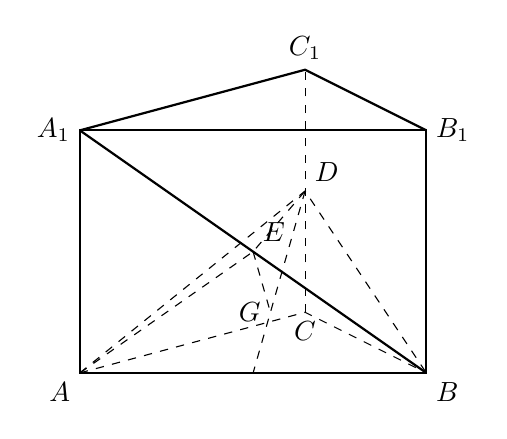
\begin{tikzpicture}[>=stealth,scale=1.1]
  % Vertices
  \coordinate (A) at (0,0);
  \coordinate (B) at (4,0);
  \coordinate (A1) at (0,2.8);
  \coordinate (B1) at (4,2.8);
  \coordinate (C) at (2.6,0.7);
  \coordinate (C1) at (2.6,3.5);
  
  \coordinate (D) at (2.6,2.1); % midpoint of CC1
  \coordinate (E) at (2,1.4);   % midpoint of A1B
  
  \coordinate (M) at (2,0);     % midpoint of AB
  \coordinate (G) at (2.2,0.7); % centroid of ABD on median DM
  
  % Solid visible edges of prism
  \draw[thick] (A) -- (B) -- (B1) -- (A1) -- cycle;
  \draw[thick] (A1) -- (C1) -- (B1);
  \draw[thick] (A1) -- (B); % diagonal
  
  % Dashed edges of prism
  \draw[dashed] (A) -- (C) -- (B);
  \draw[dashed] (C) -- (D) -- (C1);
  
  % Dashed lines for problem geometry
  \draw[dashed] (A) -- (D) -- (B);
  \draw[dashed] (A) -- (E) -- (D);
  \draw[dashed] (E) -- (G);
  \draw[dashed] (D) -- (M);
  
  % Labels
  \node[below left] at (A) {$A$};
  \node[below right] at (B) {$B$};
  \node[left] at (A1) {$A_1$};
  \node[right] at (B1) {$B_1$};
  \node[below] at (C) {$C$};
  \node[above] at (C1) {$C_1$};
  \node[above right] at (D) {$D$};
  \node[above right] at (E) {$E$};
  \node[left] at (G) {$G$};
\end{tikzpicture}
\end{center}
\nopagebreak[4]
\end{question}
\begin{question}
\gkti{20}已知常数 $a > 0$，向量 $\vec{c} = (0, a)$，$\vec{i} = (1, 0)$．经过原点 $O$ 以 $\vec{c} + \lambda\vec{i}$ 为方向向量的直线与经过定点 $A(0, a)$ 以 $\vec{i} - 2\lambda\vec{c}$ 为方向向量的直线相交于 $P$，其中 $\lambda \in \mathbf{R}$．试问：是否存在两个定点 $E$、$F$，使得 $|PE| + |PF|$ 为定值．若存在，求出 $E$、$F$ 的坐标；若不存在，说明理由．

\end{question}
\begin{question}
\gkti{21}已知 $a > 0$，$n$ 为正整数．
(1) 设 $y = (x - a)^n$，证明：$y' = n(x - a)^{n-1}$；
(2) 设 $f_n(x) = x^n - (x - a)^n$，对任意 $n \ge a$，证明：$f_{n+1}'(n+1) > (n+1)f_n'(n)$．

\Needspace{0.4\textheight}
\end{question}
\begin{question}
\gkti{22}设 $a > 0$，如图，已知直线 $l: y = ax$ 及曲线 $C: y = x^2$，$C$ 上的点 $Q_1$ 的横坐标为 $a_1$ ($0 < a_1 < a$)．从 $C$ 上的点 $Q_n$ ($n \ge 1$) 作直线平行于 $x$ 轴，交直线 $l$ 于点 $P_{n+1}$，再从点 $P_{n+1}$ 作直线平行于 $y$ 轴，交曲线 $C$ 于点 $Q_{n+1}$．$Q_n$ ($n = 1, 2, 3, \cdots$) 的横坐标构成数列 $\{a_n\}$．
(1) 试求 $a_{n+1}$ 与 $a_n$ 的关系，并求 $\{a_n\}$ 的通项公式；
(2) 当 $a = 1$，$a_1 \le \dfrac{1}{2}$ 时，证明：$\sum_{k=1}^n (a_k - a_{k+1}) a_{k+2} < \dfrac{1}{32}$；
(3) 当 $a = 1$ 时，证明：$\sum_{k=1}^n (a_k - a_{k+1}) a_{k+2} < \dfrac{1}{3}$．
\nopagebreak[4]
\begin{center}% 2003 年江苏卷第 22 题：直线与曲线迭代蛛网图
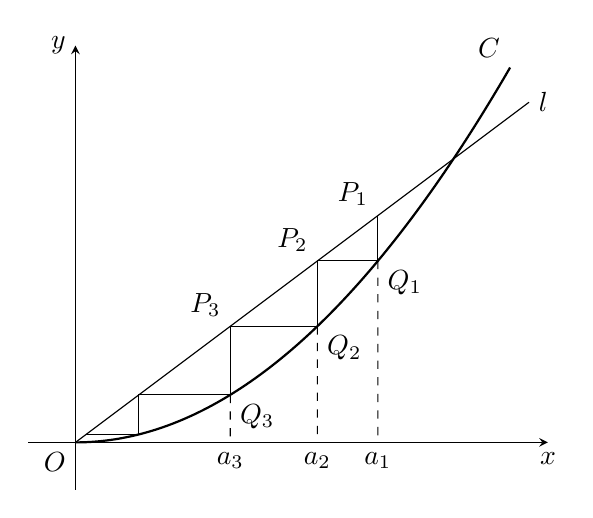
\begin{tikzpicture}[>=stealth,scale=1.2]
  % Parameters
  \def\slopeL{0.75}
  \def\cParab{0.1875} % 3.0 / 16.0
  
  \def\aOne{3.2}
  \def\aTwo{2.56}
  \def\aThree{1.6384}
  \def\aFour{0.671}
  
  % Coordinates of staircase
  \coordinate (P1) at (\aOne, {\slopeL*\aOne});
  \coordinate (Q1) at (\aOne, {\cParab*\aOne*\aOne});
  
  \coordinate (P2) at (\aTwo, {\cParab*\aOne*\aOne});
  \coordinate (Q2) at (\aTwo, {\cParab*\aTwo*\aTwo});
  
  \coordinate (P3) at (\aThree, {\cParab*\aTwo*\aTwo});
  \coordinate (Q3) at (\aThree, {\cParab*\aThree*\aThree});
  
  \coordinate (P4) at (\aFour, {\cParab*\aThree*\aThree});
  \coordinate (Q4) at (\aFour, {\cParab*\aFour*\aFour});
  \coordinate (P5) at ({\cParab*\aFour*\aFour / \slopeL}, {\cParab*\aFour*\aFour});
  
  % Axes
  \draw[->] (-0.5,0) -- (5.0,0) node[below] {$x$};
  \draw[->] (0,-0.5) -- (0,4.2) node[left] {$y$};
  \node[below left] at (0,0) {$O$};
  
  % Line l
  \draw (0,0) -- (4.8, {4.8*\slopeL}) node[right] {$l$};
  
  % Curve C
  \draw[thick, domain=0:4.6, samples=100] plot (\x, {\cParab*\x*\x}) node[above left] {$C$};
  
  % Staircase
  \draw (P1) -- (Q1) -- (P2) -- (Q2) -- (P3) -- (Q3) -- (P4) -- (Q4) -- (P5);
  
  % Dashed projections to x axis
  \draw[dashed] (Q1) -- (\aOne, 0) node[below] {$a_1$};
  \draw[dashed] (Q2) -- (\aTwo, 0) node[below] {$a_2$};
  \draw[dashed] (Q3) -- (\aThree, 0) node[below] {$a_3$};
  
  % Labels
  \node[above left] at (P1) {$P_1$};
  \node[above left] at (P2) {$P_2$};
  \node[above left] at (P3) {$P_3$};
  \node[below right] at (Q1) {$Q_1$};
  \node[below right] at (Q2) {$Q_2$};
  \node[below right] at (Q3) {$Q_3$};
\end{tikzpicture}
\end{center}
\nopagebreak[4]

\end{question}